\documentclass{article}

% if you need to pass options to natbib, use, e.g.:
\PassOptionsToPackage{numbers, compress}{natbib}
% before loading neurips_2026

\usepackage[preprint]{neurips_2026}
\usepackage[utf8]{inputenc} % allow utf-8 input
\usepackage[T1]{fontenc}    % use 8-bit T1 fonts
\usepackage{hyperref}       % hyperlinks
\usepackage{url}            % simple URL typesetting
\usepackage{booktabs}       % professional-quality tables
\usepackage{amsmath}        % math environments and operators
\usepackage{amsfonts}       % blackboard math symbols
\usepackage{nicefrac}       % compact symbols for 1/2, etc.
\usepackage{microtype}      % microtypography
\usepackage{xcolor}         % colors
\usepackage{amsthm}
\usepackage{graphicx}

\newtheorem{theorem}{Theorem}

\title{Reinforcement Learning for Adaptive Defense in Multi-Agent LLM Systems \\ \vspace{0.5em} \Large Project Milestone \\ \large Team 10}

\author{%
  Ruiteng Li \\
  \texttt{ruitengl@usc.edu} \\
  \And
  Shi He \\
  \texttt{shihe@usc.edu} \\
  \And
  Congkang Lyu \\
  \texttt{congkang@usc.edu} \\
}

\begin{document}

\maketitle

\section{Introduction}
In large language model multi-agent systems ({LLM-MAS}), multiple agents collaborate through natural language to solve complex tasks \citep{wang2024survey, xi2023rise}. Frameworks such as {AutoGen} \citep{wu2023autogen}, {CAMEL} \citep{li2023camel}, and {MetaGPT} \citep{hong2023metagpt} demonstrate how role-based {LLM} agents can collaborate. While these systems enable scalable reasoning, they implicitly assume that inter-agent communication is trustworthy. The \textit{Agent-in-the-Middle ({AiTM})} threat model \citep{he2025redteaming} considers an adversary that intercepts and manipulates messages exchanged between otherwise benign agents. Classical Byzantine fault-tolerant ({BFT}) protocols assume deterministic state machines \citep{lamport1982byzantine, zheng2025bft}. This assumption does not hold in {LLM-MAS}, where agents are inherently stochastic and may produce diverse outputs even under identical inputs.

Using a static redundancy level $k$ across every message becomes inefficient when attack intensity changes over time and communication bandwidth is constrained. We therefore ask whether reinforcement learning can learn an adaptive policy that improves message-integrity success at the same average communication budget.

\section{Methodology}
\paragraph{Communication-layer defense.}
The defense mitigates {AiTM} attacks by replicating each message across $k$ independent logical routes (where $k$ is odd). At most two routes carry the full message payload along with its hash, while the remaining routes carry only 64-byte cryptographic hash witnesses. Let $C(H^*)$ denote the frequency of the most frequent hash value. A quorum is achieved if $C(H^*) > k/2$. Under a bounded adversary controlling fewer than half of the communication routes, the defense guarantees that tampered messages cannot be accepted.

\paragraph{Adaptive controllers.}
All four methods select a redundancy level $k_t \in \mathcal{K} = \{1, 3, 5, 7\}$. The first transmission preserves message integrity when $A_t < (k_t + 1)/2$, where $A_t$ is the number of attacked replicas. If the first transmission fails, the attack is resampled within the same stage and at most one retry is allowed. All four methods share this common retry rule; retry is not a separate learned action.

We compare a fixed baseline, stateless {ML} using message length and importance, stateful {ML} using a $7$-nearest-neighbor classifier, and linear Q-learning {RL}. Stateful {ML} and {RL} receive the same $12$-dimensional feature vector $\phi(x_t)$. Historical statistics are computed from simulation feedback of completed rounds, and decisions never access the current hidden stage.

\paragraph{Cost and objective.}
For a message of length $L_t$, at most two replicas carry the full text and additional replicas carry $64$-byte hashes. One transmission sends
\[
B(k, L) = \min(k, 2)L + \max(0, k - 2) \times 64\ \text{bytes}.
\]
We treat single-copy transmission $B(1, L)$ as the baseline cost. The extra bytes for a $100$-byte message at redundancy $3$ define the normalization unit:
\[
B_{\mathrm{ref}} = B(3, 100) - B(1, 100) = 164\ \text{bytes}.
\]
For retry count $n_t \in \{0, 1\}$, the normalized communication cost and episode average are
\begin{equation}
c_t^{\mathrm{comm}} = \frac{B(k_t, L_t) - B(1, L_t) + n_t B(k_t, L_t)}{B_{\mathrm{ref}}}, \qquad
\bar{C} = \frac{1}{T}\sum_{t=1}^{T} c_t^{\mathrm{comm}}.
\label{eq:comm_cost}
\end{equation}
Equation~\eqref{eq:comm_cost} counts both initial redundancy and post-failure retries in a common unit across message lengths. Here $\bar{C} = 1$ corresponds to $164$ extra bytes per round under the reference setting, rather than one transmission or one additional copy.

Following \citet{nyberg2023learning}, who model defense expenditure and compromise losses separately, let $S_t$ indicate final success after any retry. Message importance takes values $\omega_t \in \{0.5, 1.0, 1.5\}$ to represent losses from final delivery failures. The reward and optimization objective are
\[
r_t = -c_t^{\mathrm{comm}} - \omega_t (1 - S_t), \qquad
\max_{\pi}\ \mathbb{E}_{\pi}\left[\sum_{t=1}^{T} \gamma^{t-1} r_t\right].
\]
Equal nominal budgets $b$ do not yield equal average costs $\bar{C}$. We therefore sweep $b$ and interpolate within the measured cost range covered by all four methods to compare success rates at matched $\bar{C}$.

\section{Preliminary Results}
\paragraph{Static routing.}
The baseline system uses Qwen2.5-14B in a two-agent setup (Coder and Reviewer) with no communication defenses. We simulate an {AiTM} adversary with $\alpha = 0.33$ control over the network. Without the defense, {AiTM} attacks had a $100\%$ Attack Success Rate ({ASR}) on MBPP. With the defense enabled ($k=3$), the {ASR} dropped to $0.0\%$ across all $427$ tasks. System availability remained at $100\%$.

\paragraph{Adaptive redundancy setup.}
Our adaptive redundancy experiments currently run in a numerical simulator. The attack model has three stages: \emph{quiet}, \emph{probing}, and \emph{burst}. The multiple-attacker experiment uses three independent stochastic processes activated at round $0$, approximately $T/3$, and approximately $2T/3$. Episodes have $180$ rounds; random seeds are $7, 42, 99$. Training uses $1{,}000$ episodes per budget and seed for each learned method; evaluation uses $10$ test episodes per method, budget, and seed. Controllers are trained separately for each nominal budget and random seed, using distinct seed offsets between training and evaluation. Across the two attack conditions, we complete $42$ training-and-evaluation configurations, evaluating the four methods over $1{,}680$ test episodes ($302{,}400$ message rounds in total).

\begin{table}[t]
\centering
\small
\caption{Message-integrity success rates (\%) at matched average communication cost $\bar{C} = 1.0$ (mean $\pm$ approximate $95\%$ confidence interval half-width).}
\label{tab:matched_cost}
\begin{tabular}{lrr}
\toprule
\textbf{Method} & \textbf{One Attacker (\%)} & \textbf{Three Attackers (\%)} \\
\midrule
Fixed baseline & $86.31 \pm 2.68$ & $60.37 \pm 1.60$ \\
Stateless {ML} & $88.62 \pm 2.16$ & $70.54 \pm 0.78$ \\
Stateful {ML}  & $\mathbf{88.64 \pm 2.13}$ & $70.45 \pm 0.79$ \\
Q-learning {RL} & $88.43 \pm 1.64$ & $\mathbf{78.52 \pm 0.54}$ \\
\bottomrule
\end{tabular}
\end{table}

Results for each seed are interpolated along the measured average communication-cost axis $\bar{C}$ and then averaged across the three seeds. Intervals in Table~\ref{tab:matched_cost} show $\bar{p} \pm 1.96\,s/\sqrt{3}$; these summarize variation across seeds rather than significance tests.

Under one attacker, {RL} and both {ML} methods achieve similar success rates. Under three staggered attackers at $\bar{C} = 1.0$, Q-learning {RL} reaches $78.52\%$, exceeding Stateless {ML} ($70.54\%$) by $7.98$ percentage points and the fixed baseline ($60.37\%$) by $18.15$ percentage points. Stateful {ML} ($70.45\%$) and Stateless {ML} ($70.54\%$) perform nearly identically. The single-attacker results do not support a general claim that {RL} consistently outperforms {ML}.

\begin{figure}[htbp]
\centering
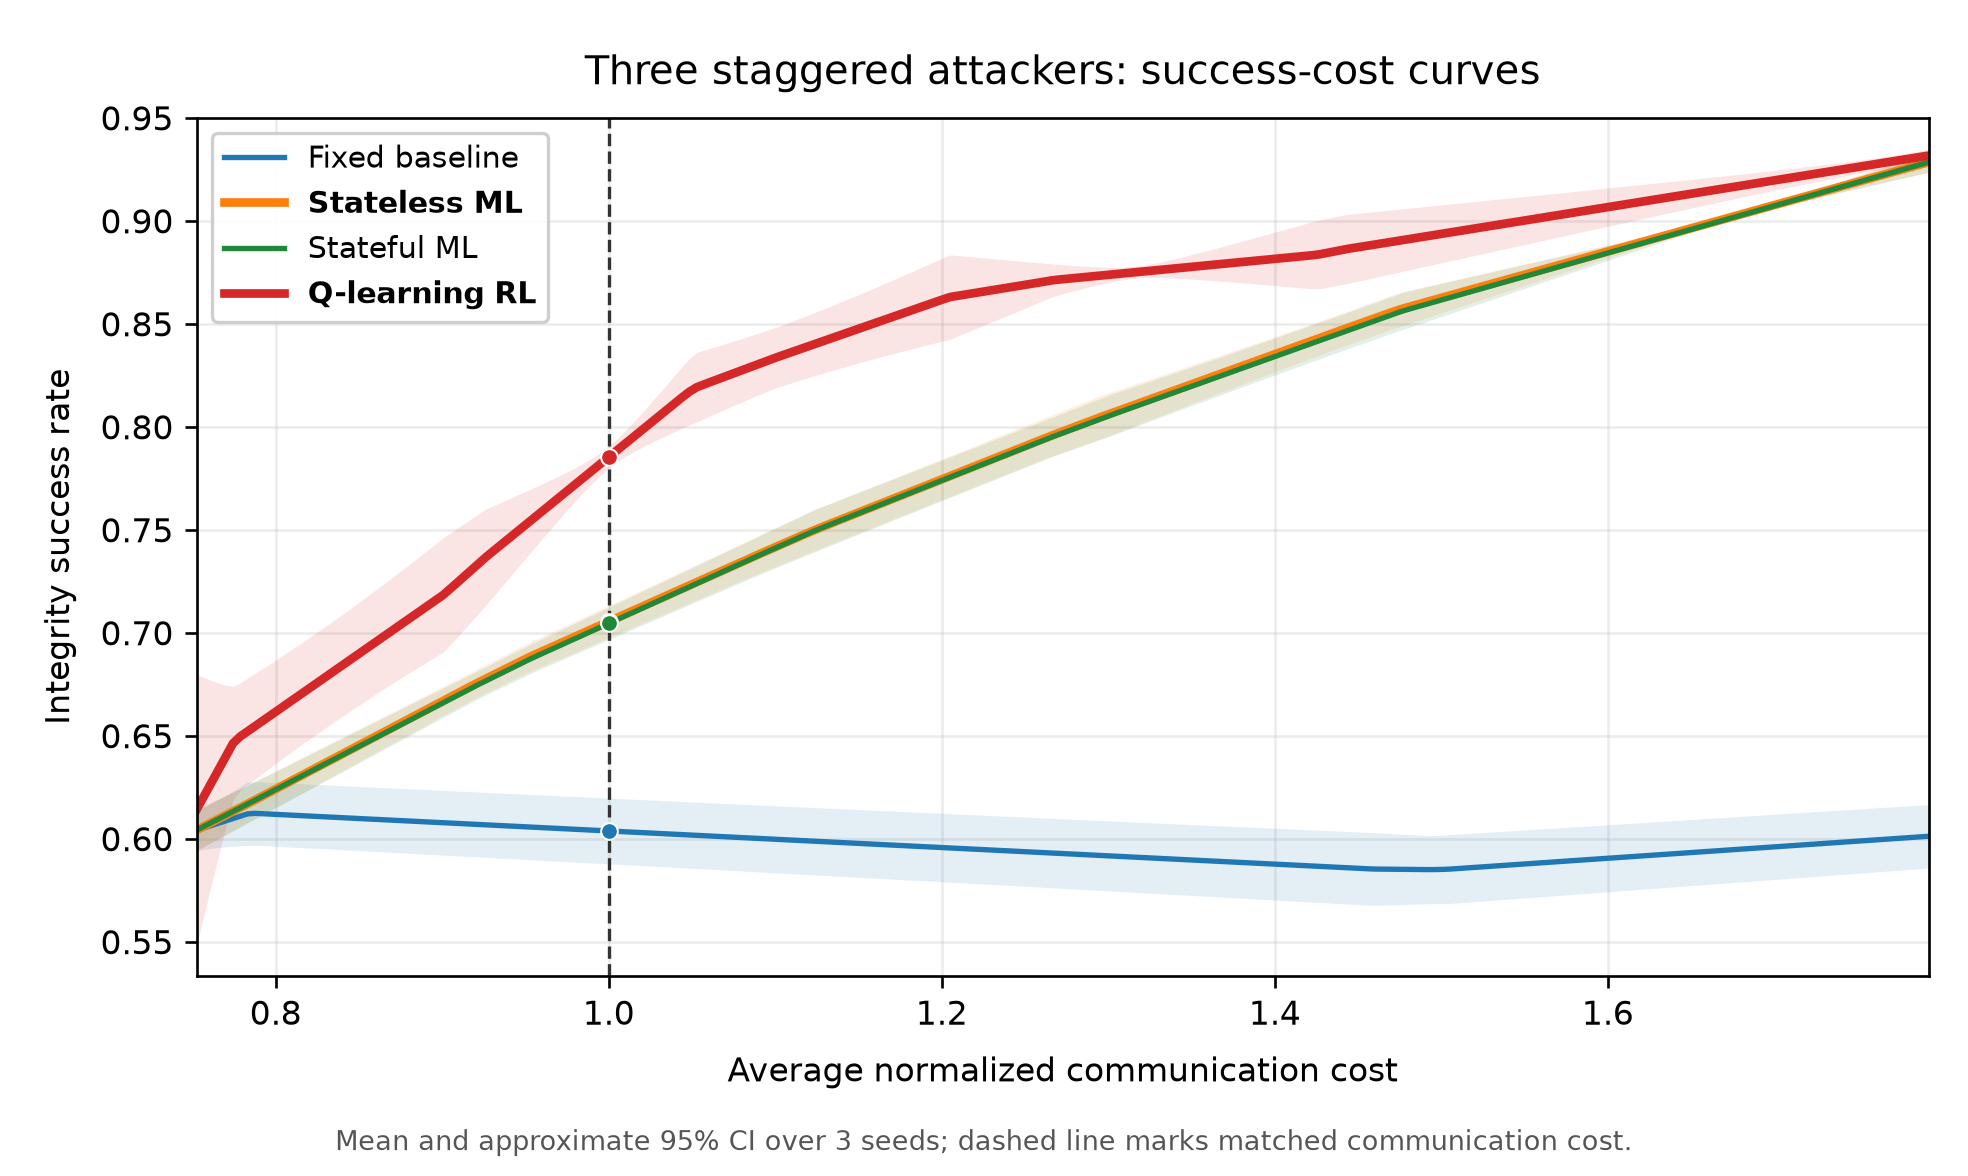
\includegraphics[width=0.78\linewidth]{figures/02_multiple_attackers_success_cost.png}
\caption{Three staggered attackers. Q-learning {RL} achieves higher success rates in the intermediate-cost range, and the gap between {ML} and {RL} narrows as communication cost increases. The dashed line marks an average cost of $1.0$.}
\label{fig:multi_attacker}
\end{figure}

\begin{figure}[htbp]
\centering
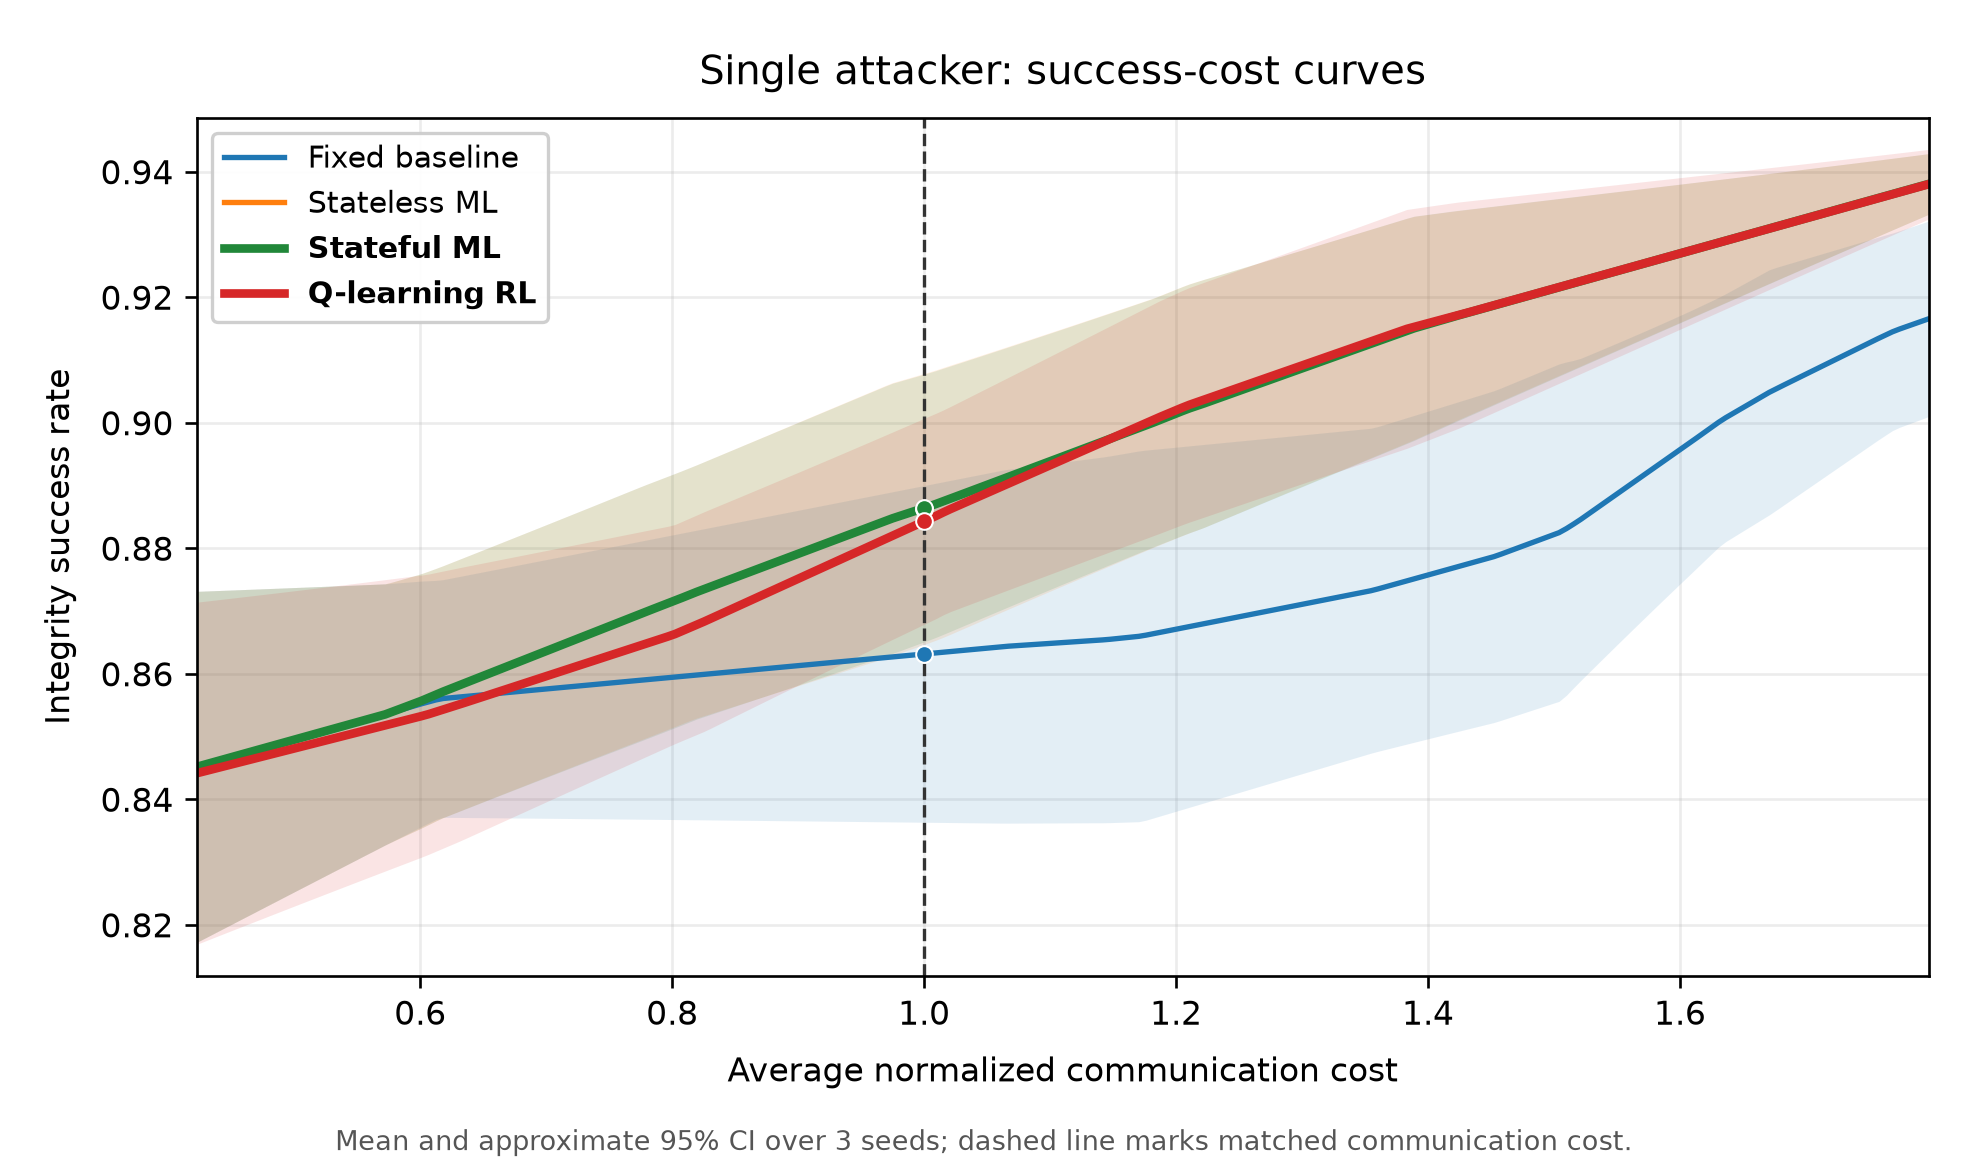
\includegraphics[width=0.78\linewidth]{figures/01_single_attacker_success_cost.png}
\caption{Single-attacker condition. The three learned methods produce similar curves and outperform the fixed baseline near an average communication cost of $1.0$ (dashed line).}
\label{fig:single_attacker}
\end{figure}

\section{Plan Until the Final Report}
\begin{itemize}
\item \textbf{Week 1:} Reformulate the simulator as a partially observable decision process ({POMDP}) with noisy pre-transmission risk alerts, persistent channel compromise, and independent multi-attacker target unions.
\item \textbf{Weeks 2--3:} Compare our linear Q-learning baseline against deep {RL} algorithms and supervised {ML} classifiers on identical observations. Train candidate policies using domain randomization, soft budget constraints, and multi-attacker schedules.
\item \textbf{Week 4:} Construct success--cost frontiers to compare methods at matched average cost across $1$--$5$ attackers. Run multi-factor stress tests, perform minimal closed-loop integration into the live {LLM-MAS} communication layer, and complete statistical uncertainty analysis for the final report.
\end{itemize}

\clearpage
\bibliographystyle{plainnat}
\bibliography{references}
\clearpage
\appendix
\section*{Appendix}
\section{Team Contributions}
Each member contributed one third of the project work:
\begin{itemize}
    \item \textbf{Ruiteng Li:} Communication-layer defense, quorum verification, and integration with the multi-agent frameworks.
    \item \textbf{Shi He:} Attack and workload simulation, adaptive {ML}/{RL} controllers, and budget and reward formulation.
    \item \textbf{Congkang Lyu:} Experimental evaluation, matched-cost comparisons, uncertainty analysis, and result figures and tables.
\end{itemize}
All three jointly prepared the report.

\section{Technical Details}
\begin{theorem}
Let $k$ be an odd number of communication routes, and let $\alpha < 0.5$ denote the fraction of routes controlled by a Byzantine adversary. The defense guarantees that no tampered message can be accepted by the receiving agent.
\end{theorem}
\textbf{Proof sketch.} Since $\alpha < 0.5$, strictly more than half of the routes are honest. All honest routes report identical hashes corresponding to the correct message $m$. An adversary controlling fewer than half of the routes cannot produce a matching majority for a tampered message $m'$.

\subsection{Ghost Channels for Dynamic Routing}
Drawing inspiration from Moving Target Defense ({MTD}) \citep{skowyra2020mtd, jailbreaker2024}, the defense introduces \textit{Ghost Channels}. When quorum inconsistencies are detected, compromised routes are dynamically replaced with new logical routes, re-randomizing the communication structure over time.

\subsection{Attack and Workload Modeling}
\citet{liao2020network} use a hidden Markov model ({HMM}) to describe transitions among safe, probing, attack, and compromised states. Following this modeling approach, we simplify attacker behavior into three stages: \emph{quiet}, \emph{probing}, and \emph{burst}. Stages may persist, escalate, or retreat under the base transition matrix
\[
P_{ij} = \Pr(z_{t+1} = j \mid z_t = i), \qquad
P = \begin{bmatrix}
0.90 & 0.09 & 0.01 \\
0.10 & 0.75 & 0.15 \\
0.05 & 0.10 & 0.85
\end{bmatrix}.
\]
Attack probability depends on the stage via $I_t \sim \operatorname{Bernoulli}(p_{z_t})$. The number of replicas attacked by one attacker is
\[
A_t = I_t \min\{3, 1 + N_t\}, \qquad N_t \sim \operatorname{Poisson}(\lambda_{z_t}),
\]
where $p = (0.02, 0.20, 0.75)$ and $\lambda = (0, 0.5, 2.0)$ for the three stages. Both $P$ and $(p, \lambda)$ are experimental settings, and stages do not follow a fixed sequence.

The multiple-attacker experiment uses three independent stochastic processes activated at round $0$, approximately $T/3$, and approximately $2T/3$. The latter two activation times receive integer random perturbations within $[-T/12, T/12]$. Attacked replica counts in each round follow a conservative additive cap:
\[
A_t^{\mathrm{multi}} = \min\left\{3, \sum_{j=1}^{3} \mathbf{1}[t > \tau_j]\, A_t^{(j)}\right\}.
\]
Each attacker maintains its own state and random number stream while sharing recent defense outcomes as feedback. A predefined rule increases the probability of entering probing and burst stages when recent defense success drops; the attackers themselves are not trained.

Message workloads follow three persistent states with reference lengths of $50$, $100$, and $200$ bytes. Random perturbations and temporal smoothing produce gradual length changes across rounds. Message importance takes values $\omega_t \in \{0.5, 1.0, 1.5\}$ to represent losses from final delivery failures.

\subsection{Controller Features and Updates}
\begin{table}[t]
\centering
\small
\caption{Comparison of the four redundancy selection methods.}
\label{tab:methods}
\begin{tabular}{@{}p{0.20\linewidth} p{0.38\linewidth} p{0.35\linewidth}@{}}
\toprule
\textbf{Method} & \textbf{Decision Rule} & \textbf{Inputs and Learning Objective} \\
\midrule
Fixed baseline & Uses a fixed target redundancy, subject to the remaining budget & Basic resource-allocation reference \\
Stateless {ML} & Groups messages by length and importance and outputs the modal supervised action label & Does not use attack history \\
Stateful {ML} & Predicts actions with a $7$-nearest-neighbor classifier & Uses historical features to fit labels minimizing local cost \\
Q-learning {RL} & Selects actions via a linear approximation of Q-values & Optimizes cumulative return over sequential interactions \\
\bottomrule
\end{tabular}
\end{table}

Table~\ref{tab:methods} summarizes the four controllers. Stateful {ML} and {RL} receive the same $12$-dimensional feature vector $\phi(x_t)$. It contains short- and long-term attack statistics, attack frequency, time since the last attack, episode progress, remaining budget, message length, importance, and interaction terms. Historical statistics are computed from simulation feedback of completed rounds, and decisions never access the current hidden stage.

Supervised labels are generated from simulated single-step communication costs and failure losses, with Stateful {ML} retaining at most $3{,}000$ training samples. The {RL} action-value approximation and update are
\[
Q(x_t, k) = w_k^\top \phi(x_t), \qquad
\delta_t = r_t + \gamma \max_{k' \in \mathcal{K}_{t+1}} Q(x_{t+1}, k') - Q(x_t, k_t),
\]
\[
w_{k_t} \leftarrow w_{k_t} + \alpha \operatorname{clip}(\delta_t, -5, 5)\,\phi(x_t),
\]
where $\mathcal{K}_{t+1} \subseteq \mathcal{K}$ contains actions permitted by the remaining budget and terminal future value is zero.

Training and evaluation also impose a shared redundancy-capacity constraint: each action consumes $d(k) = (k - 1)/2$ units, and each episode must consume its exact capacity $\operatorname{round}(bT)$. Because message lengths and retry counts vary, equal nominal budgets $b$ do not yield equal average costs $\bar{C}$. We therefore sweep $b$ and interpolate within the measured cost range covered by all four methods to compare success rates at matched $\bar{C}$.

\section{Additional Experimental Details}
\subsection{Experimental Setup}
Our preliminary evaluations focus on coding and reasoning tasks using the MBPP, HumanEval, and MMLU benchmarks. We use Qwen2.5-14B as our base model for the preliminary static routing experiments. The baseline system consists of a standard two-agent setup (Coder and Reviewer) with no communication defenses, while the hardened system routes all messages through the defense with $k=3$ and $k=5$ configurations. We simulate an AiTM adversary with $\alpha = 0.33$ control over the network.

\subsection{Initial Failures and Edge Cases}
During early testing, we observed a failure mode where legitimate, non-malicious stochastic variations in API routing caused hash mismatches. We resolved this by moving the hashing mechanism strictly to the payload content prior to transport serialization. Transmitting the full text across all $k$ routes introduced unnecessary network bandwidth overhead. We mitigated this using our asymmetric hash-only route design.

\subsection{Adaptive Redundancy Experimental Parameters}
Table~\ref{tab:params} summarizes the simulation parameters for our adaptive redundancy experiments. Controllers are trained separately for each nominal budget and random seed, using distinct seed offsets between training and evaluation. Across the two attack conditions, we complete $42$ training-and-evaluation configurations, evaluating the four methods over $1{,}680$ test episodes ($302{,}400$ message rounds in total).

\begin{table}[t]
\centering
\small
\caption{Parameters for the adaptive redundancy defense experiments.}
\label{tab:params}
\begin{tabular}{ll}
\toprule
\textbf{Parameter} & \textbf{Setting} \\
\midrule
Attack conditions & One attacker; three attackers with staggered activation times \\
Attack model & Three-stage bursty {HMM} \\
Episode length & $180$ rounds \\
Training per budget and seed & $1{,}000$ supervised episodes ({ML}); $1{,}000$ training episodes ({RL}) \\
Evaluation per method & $10$ independent test episodes per budget and seed \\
Random seeds & $7,\ 42,\ 99$ \\
Nominal capacity budget $b$ & $0.25,\ 0.50,\ 0.75,\ 1.00,\ 1.25,\ 1.50,\ 2.00$ \\
History window & $30$ rounds \\
Q-learning parameters & Learning rate $\alpha = 0.01$; discount factor $\gamma = 0.99$ \\
\bottomrule
\end{tabular}
\end{table}

Message-integrity success is computed as
\[
\hat{p}_{\mathrm{success}} = \frac{\sum_{e, t} S_{e, t}}{\sum_e T_e}.
\]
Results for each seed are interpolated along the measured average communication-cost axis $\bar{C}$ and then averaged across the three seeds. Shaded bands in Figures~\ref{fig:multi_attacker} and~\ref{fig:single_attacker} and intervals in Table~\ref{tab:matched_cost} show $\bar{p} \pm 1.96\, s / \sqrt{3}$; these intervals summarize variation across seeds under the given configuration rather than significance tests.

\section{Additional Related Work}

\subsection{Security Defenses in {LLM-MAS}}
Current approaches predominantly focus on endpoint hardening. Prior work has identified vulnerabilities such as malfunction amplification \citep{zhang2024breaking}. Specifically, \citet{zhang2024breaking} show that relying on {LLM}-based self-examination is often ineffective. At the system level, approaches attempt to resolve inconsistencies through inter-agent debate \citep{xiong2023inter, amayuelas2024multiagent}. \citet{he2025redteaming} formalize this vulnerability through the {AiTM} attack, demonstrating that adversaries can manipulate multi-agent workflows in transit.

\subsection{Byzantine Fault Tolerance ({BFT}) and {MTD}}
{BFT} provides a classical framework for securing distributed systems \citep{lamport1982byzantine}. Recent work by \citet{zheng2025bft} adapts {BFT} concepts to {LLM}-based systems by leveraging model-internal reasoning. Moving Target Defense ({MTD}) techniques dynamically alter system configurations \citep{skowyra2020mtd}, recently applied to prompt-level {LLM} security \citep{jailbreaker2024}. The defense combines these paradigms, applying {BFT} principles to opaque message payloads and extending {MTD} to the communication topology via Ghost Channels.

\subsection{Attack Modeling and {RL} for Adaptive Cyber Defense}
\citet{liao2020network} model network security situation changes across safe, probing, attack, and compromised hidden states using an extended hidden Markov model. We build on this hidden-stage abstraction to generate time-varying attack intensity. On the defender side, \citet{nyberg2023learning} learn automated defense strategies in graph-based cyber attack simulations by separating defense activation cost from target-compromise loss, motivating our separate communication-cost and failure-loss reward formulation.


\end{document}
